% PLEASE USE THIS FILE AS A TEMPLATE
% Check file iosart2c.tex for more examples
%
% Journal:
%   Journal of Ambient Intelligence and Smart Environments (jaise)
%   Web Intelligence and Agent Systems: An International Journal (wias)
%   Semantic Web: Interoperability, Usability, Applicability (SW)
% IOS Press
% Latex 2e

% options: jaise|wias|sw
% add. options: [seceqn,secfloat,secthm,crcready,onecolumn]


%\documentclass{iosart2c}

\documentclass[sw]{iosart2c}
%\documentclass[wias]{iosart2c}
%\documentclass[jaise]{iosart2c}

\usepackage[T1]{fontenc}
\usepackage[utf8]{inputenc}

\usepackage{times}%
\usepackage{natbib}% for bibliography sorting/compressing
%\usepackage{amsmath}
%\usepackage{endnotes}
%\usepackage{graphics}

%%%%%%%%%%% Put your definitions here
\usepackage{url}
\usepackage{graphicx}

\usepackage{ccicons}
\usepackage{relsize}
\newcommand{\uri}[1]{\textsf{\textscale{0.9}{#1}}}
%\newcommand{\uri}[1]{\textsf{\small{#1}}}
%%%%%%%%%%% End of definitions

\pubyear{0000}
\volume{0}
\firstpage{1}
\lastpage{1}

\begin{document}

\begin{frontmatter}

%\pretitle{}
\title{Dbnary: Wiktionary as a Lemon Based RDF Multilingual Lexical Ressource}
\runningtitle{Dbnary}
%\subtitle{}

%\review{}{}{}


% For one author:
\author{\fnms{Gilles} \snm{Sérasset}\thanks{E-mail: Gilles.Serasset@imag.fr.}}
\address{GETALP-LIG, UJF-Grenoble 1 \\BP 53, 38051 Grenoble cedex 9, France\\ \texttt{gilles.serasset@imag.fr}}
\runningauthor{Gilles Sérasset}

% Two or more authors:
%\author[A]{\fnms{} \snm{}\thanks{}},
%\author[B]{\fnms{} \snm{}}
%\runningauthor{}
%\address[A]{}
%\address[B]{}

\begin{abstract}
Contributive resources, such as wikipedia, have proved to be valuable in Natural Language Processing or Multilingual Information Retrieval applications. This work focusses on Wiktionary, the dictionary part of the collaborative resources sponsored by the \emph{Wikimedia} foundation. In this article, we present our effort to extract Multilingual Lexical Data from wiktionary data and to provide it to the community as a Multilingual Lexical Linked Open Data (MLLOD). This lexical resource is structured using the LEMON Model.\\
This data, called \textit{dbnary}, is registered at \url{http://thedatahub.org/dataset/dbnary}.
\end{abstract}

\begin{keyword}
Wiktionary \sep Multilingual \sep Lexical Resource \sep LEMON \sep Multilingual Linguistic LOD
\end{keyword}

\end{frontmatter}

\section{Introduction}

The GETALP (Study group for speech and language translation/processing) team of the LIG (Laboratoire d'Informatique de Grenoble) is in need for multilingual lexical resources that should include language correspondences (translations) and word sense definitions. In this regard, the data included in the different wiktionary\footnote{\url{http://www.wiktionary.org}} language edition is a precious mine.

Alas, many inconsistencies, errors, difference in usage do exist in the different wiktionary language edition. Hence, we decided to provide an effort to extract precious data from this source and provide it to the community as Linked Data. After a first version that used an RDF version of the LMF model \cite{FRANCOPOULO:2006:INRIA-00121468:1,francopoulo-EtAl:2006:MLRI} and described in \cite{serasset:lrec2012}, we decided to adapt our extractors to LEMON model \cite{McRae-lemon:2012}. This linked dataset has won the ``Monnet-Challenge'' in 2012.

\section{Extracting data from wiktionary}

\subsection{Motivation}

Errors and incoherence are inherent to a contributive resource like wiktionary. Some language editions (like French and English) have many moderators that do limit the number of incoherence among entries of the same language. Moreover, such languages, which contain the most data, use many \textit{templates} that simplify the extraction process. For instance, the translation section of the French dictionary usually uses a template to identify each individual translation.

This is not true anymore with less developed wiktionary language editions. For instance, in the Finnish edition, some translations are introduced by a template giving the language (e.g. \{fr\} precedes French translations) and others are introduced by the string "ranska" which is the Finnish translation for "French". In this case the extractor needs to know the Finnish translation of all language names to cope with the second case and avoid losing almost half of the available translation data.

Many such inconsistencies and some errors in the data renders the development of an extractor quite tedious. as many people in NLP is trying to use this data for different applications, we decided that we would extract as much data as we can from wiktionary and provide it to the community while ensuring interoperability with other lexical data.

The dbnary extractor is written in java and is open-source (LGPL licensed, available at \url{http://dbnary.forge.imag.fr}). Anyone way contribute to this extraction effort by taking contact with the author.

\subsection{Scope of the extracted data}

The main goal of our efforts is not to extensively reflect wiktionary data, but to create a lexical resource that is structured as a set of monolingual dictionaries + bilingual translation information. Such data is already useful for several application, but it is merely a starting point for a future multilingual lexical database.

The monolingual data is always extracted from its own wiktionary language edition. For instance, the French lexical data is extracted from French language edition\footnote{We use the term ``French language edition'' to refer to the data available on \url{http://fr.wiktionary.org}}. Hence, we completely disregard the French data that may be found in other language editions.

We also filtered out some part of speeches in order to produce a result that is closer to existing monolingual dictionaries. For instance, in French, we disregard abstract entries that are prefixes, suffixes or flexions (e.g.: we do not extract data concerning \textit{in-} or \textit{-al} that are prefixes/suffixes and have a dedicated page in French language edition). 

Our work did focus only on the lexical data. Hence, we do not provide any reference to any ontology.

\subsection{Availability of the extracted data}

Dbnary data is provided using Creative Commons Attribution-ShareAlike 3.0 license (\ccbysa). It may be downloaded from the dbnary website\footnote{\url{http://kaiko.getalp.org/about-dbnary}} as a set of turtle files (one per language).

As the wiktionary language editions constantly evolve with entries modifications and additions, the dbnary also evolves. Each time the wikimedia foundation provides a new dump\footnote{dumps are available at \url{http://dumps.wikimedia.org/}.} of a wiktionary language edition, dbnary data is extracted with the new dump and made available online. At the time of writing, the dumps are updated about once every ten days for each language.

Dbnary data is also available as Linguistic Linked Open Data (LLOD). Hence, all dbnary URIs are dereferencable and a SPARQL endpoint is available at \url{http://kaiko.getalp.org/sparql}. However, as the dbnary data changes almost everyday, the data that is available this way is not necessarily up to date.

\section{Extracted Data as a LEMON Lexical Resource}

\begin{figure*}[tbp]
\resizebox{\linewidth}{!}{%
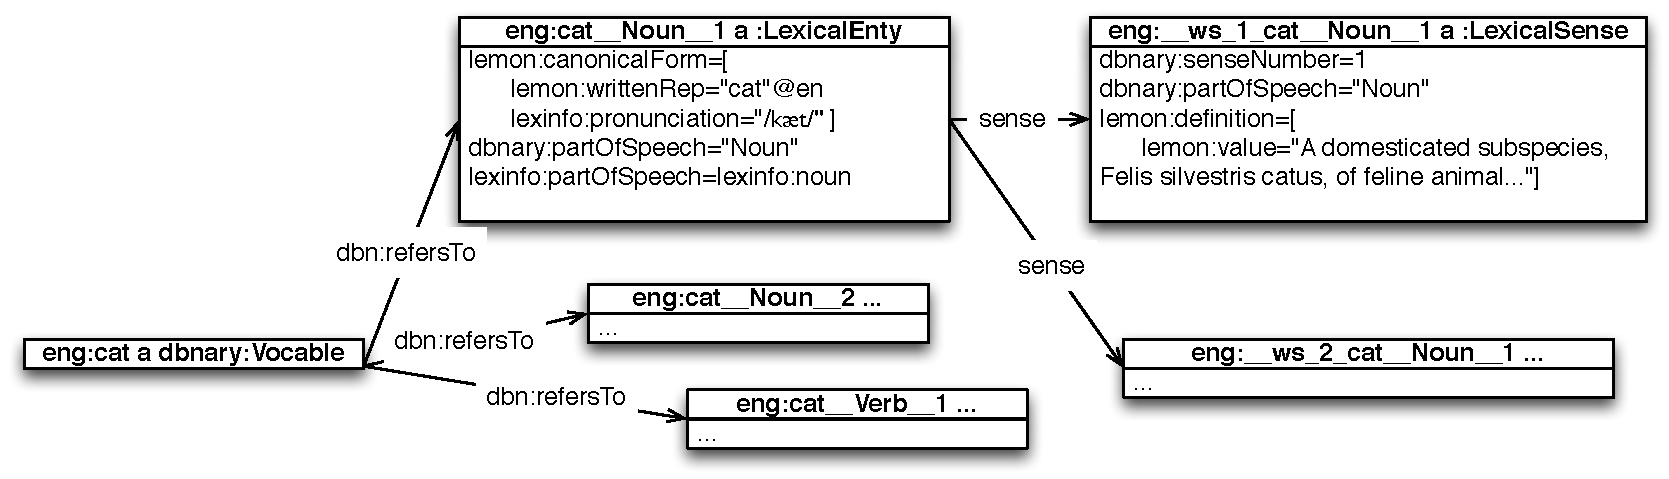
\includegraphics{cat_struct.pdf}
}
\caption{An extract of the dbnary entry "cat" in English, showing the respective roles of \uri{Vocable}, \uri{LexicalEntry} and \uri{LexicalSense} in the dbnary dataset.}\label{dbnary:cat}
\end{figure*}

\begin{figure*}[tbp]
\resizebox{\linewidth}{!}{%
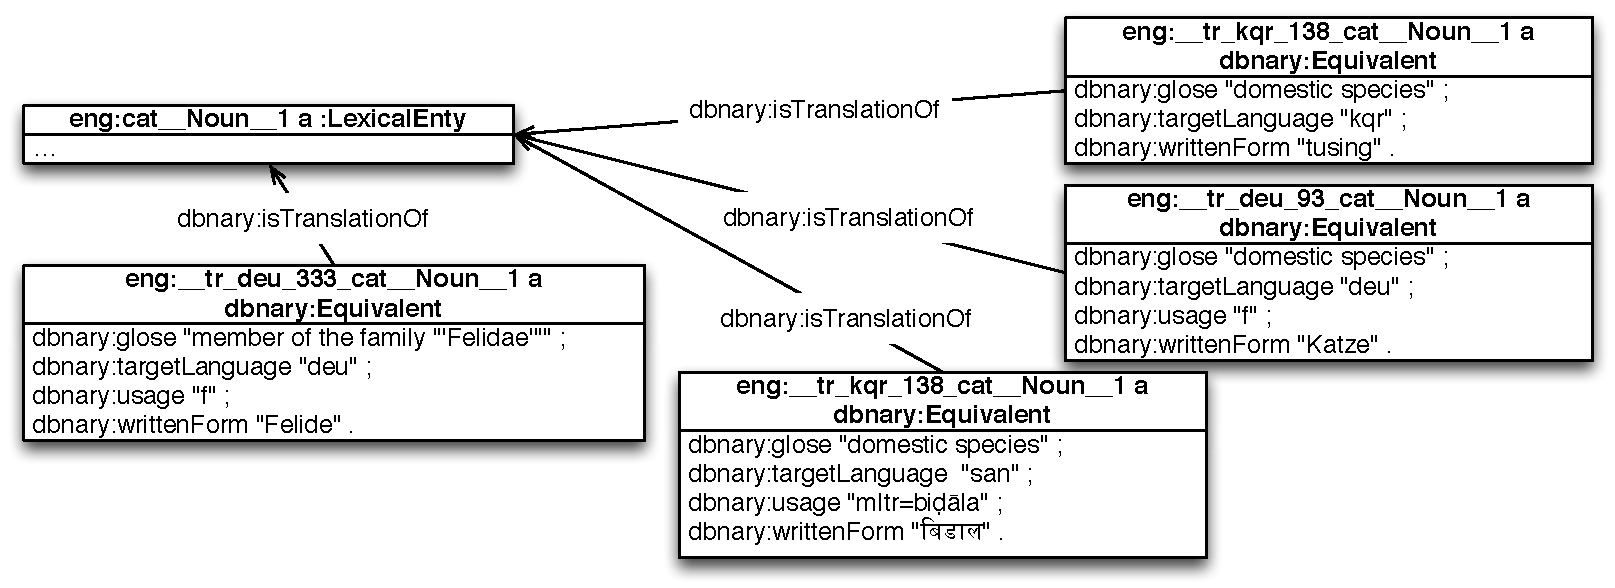
\includegraphics{cat_translations.pdf}
}
\caption{A subset of the translations related to the lexical entry \uri{eng:cat\_Noun\_1}.}\label{dbnary:catequiv}
\end{figure*}

\subsection{Using LEMON for legacy lexical data}

LEMON model itself is not sufficient to represent lexical data that is currently available in classical monolingual and bilingual dictionaries. For instance, LEMON does not contain anything to represent translations between languages as it assumes that such a translation will be handled by the ontology description. Moreover, LEMON assumes that all data is well-formed and fully specified. As an example, synonymy relation is a property linking a \uri{LexicalSense} to another \uri{LexicalSense}. While this is correct to assume as a \textit{principle}, this does not account for the huge amount of legacy data that is available in dictionaries and lexical databases.

In order to cope with this legacy data, we extended the LEMON model by adding new classes and properties. However, when a piece of data is representable as a LEMON entity, then it is done so. Moreover, when possible, we did use the ISOcat registry \cite{windhouwer2012linking} to identify standard elements in the lexical data.

\subsection{Dbnary extension to LEMON}

The LEMON model has been extended to cope with legacy lexical data. Added classes and properties are:

\begin{description}
\item[Vocable:] Several lexical entries may be contained in a single wiktionary page. And most lexical relations are simply targeted to wiktionary pages. Hence, we added the \uri{dbnary:Vocable} class to represent a wiktionary page. This class is a subclass of \uri{lemon:LexicalEntry}. Instances of this class are related to their lexical entries through the \uri{dbnary:refersTo} property. 

\item[LexicalEntity:] Lexical relations should usually link two \textit{Lexical Senses}. However, most relations found in legacy lexical data is underspecified. Some relations link a \textit{Lexical Sense} to a \textit{Vocable} or to a \textit{Lexical Entry}. Others even link two \textit{Lexical Entries}. In order to cope in a standard way with such underspecified relations, we introduced the \uri{dbnary:LexicalEntity} class which is the union of  \textit{Lexical Entry} and \textit{Lexical Sense}.

\item[Nyms:] Most wiktionary language edition do provide ``nym'' relations (mainly synonym, antonym, hypernym, hyponym, meronym and holonym), which are almost always underspecified. Hence, DBnary introduces 6 new ``nym'' properties (in \uri{dbnary} name space). These relations domains and ranges are \textit{Lexical Entities}.

\item[Translations:] As there is no way to represent bilingual translation relation in LEMON, we introduced the \uri{dbnary:Equivalent} class that collects translation information contained in wiktionary. This class admits several properties:
\begin{itemize}
\item \uri{dbnary:isTranslationOf} relates the equivalent to its source \textit{lexical Entity}. 
\item \uri{dbnary:targetLanguage} is a data property whose type is a string containing the target language code as defined in ISO639-3 standard.
\item \uri{dbnary:writtenForm} gives the written form of the translation in the target language. Here, we decided not to relate to a vocable as some translations are not to be defined as lexical entries in the target language.
\item \uri{dbnary:glose} is a string property that contains any available information used to dentate the lexical sense of the source of the equivalent.
\item \uri{dbnary:usage} is a string property that contains any available information concerning this equivalent object. It usually gives additional information on the target entry.
\end{itemize}

\end{description}

\subsection{Structure of the extracted lexical data}



Figure \ref{dbnary:cat} illustrates the main elements characterizing a lexicon entry in the dbnary data. Each wiktionary page is represented by a \uri{dbnary:Vocable} element that refers to its corresponding \uri{lemon:Lexical\-Entry}. Each lexical entry corresponds to one lemma, one etymology and one part of speech. Each lexical entry is related to its \uri{lemon:Lexical\-Sense} by the \uri{lemon:sense} property. A lexical sense corresponds to one definition. 

Each lexical entry is related to its canonical form and eventually to alternate forms (that are represented using \uri{lemon:LexicalForm}s). The part of speech is available through \uri{dbnary:partOfSpeech} property that gives the part of speech as defined by the wiktionary language edition, and through the \uri{isocat:partOfSpeech} property that points to a standard ISOcat part of speech value.

\begin{figure*}[tbp]
\resizebox{\linewidth}{!}{%
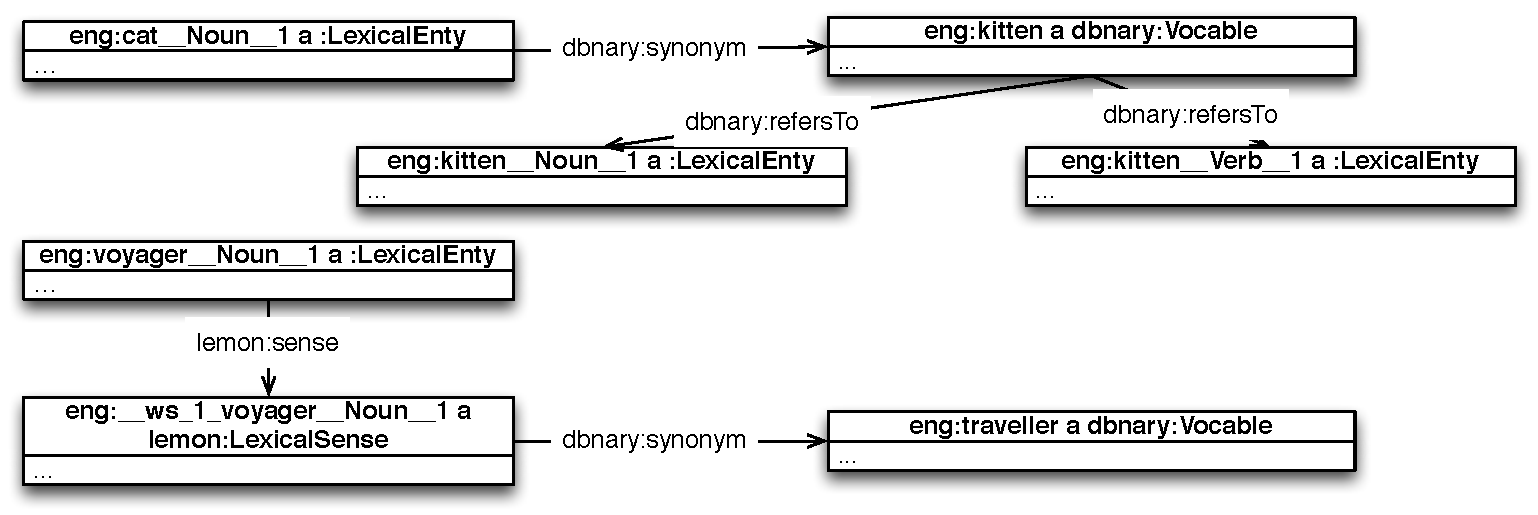
\includegraphics{cat_syn.pdf}
}
\caption{An example of a synonymy relation for the lexical entry \uri{eng:cat\_Noun\_1}.}\label{dbnary:catsyn}
\end{figure*}


Figure \ref{dbnary:catequiv} illustrates the \textit{dbnary} extension to LEMON that is used to represent the many translations that are available in wiktionary. Each translation is represented as a \uri{dbnary:Equivalent} instance that is associated to a \textit{lexical entry} by the \uri{is\-Translation\-Of} property. The translation is given as a string through the \uri{writtenForm} property, as some translations may not necessarily correspond to vocables in the target language (e.g. explanatory translations). The target language of the translation is given using ISO  639-3 3 letter language code \cite{ISO639-3:2007}. When available, the \uri{glose} property value gives an indication concerning the lexical sense that is translated. In the current dataset, the translation is linked to an usually ambiguous lexical entry and the \textit{glose} is kept for further attachment to the correct word sense.

Wiktionary contains many lexical relations (like synonymy, antonymy, etc.) that are represented using the above mentioned ``nym'' properties which relate a \textit{lexical entity} with another \textit{lexical entity}. In the current dataset, most of the property subjects are \textit{lexical entries}. However, in case of monosemous lexical entries, the synonymy relation is attached to the unique \uri{lemon:LexicalSense}. Figure \ref{dbnary:catsyn} illustrates how dbnary encodes ``nym'' relations with examples of the \uri{dbnary:synonym} property. In the upper part of the figure is an example of a \uri{dbnary:synonym} property that is related to the ambiguous lexical entry \uri{eng:cat\_\_Noun\_\_1}. The lower part shows that, in the monosemous lexical entry \uri{eng:voyager\_\_Noun\_\_1}, the \uri{dbnary:synonym} property is related to the unique lexical sense of the entry. The object of such properties are always \uri{dbnary:Vocable}.


\section{Size of the involved data}

All sizes indicated in this sections reflect the state of the dbnary data at the time of writing (December 2012). Table \ref{globalsize} give the number of resources available in dbnary.

\begin{table}[htb]
\begin{tabular}{lrrrr}
 & \textbf{Entries} & \textbf{Vocables} & \textbf{Senses} & \textbf{Equivalents}\\
 \hline
\textbf{eng} & 502493 & 481311 & 402815 & 1021430 \\
\textbf{fra} & 264803 & 274854 & 347076 & 419168 \\
\textbf{deu} & 106337 & 171517 & 90474 & 446563 \\
\textbf{fin} & 42813  & 43158 & 51297 & 114279 \\
\textbf{por} & 42042  & 43028 & 76124 & 197931 \\
\textbf{ita} & 24473  & 30568 & 34133 & 58383 \\
\end{tabular}
\caption{Number of resources by type and language, sorted by number of lexical entries.}\label{globalsize}
\end{table}

As the extraction is performed each time a wiktionary dump is available, this numbers are constantly evolving, as the wiktionary data is evolving and as the extractor itself may be improved.


Table \ref{nymsize} gives an overview of the number of lexico-semantic relations available in each language edition.

\begin{table}[htb]
\begin{tabular}{lrrrrrr}
 & \textbf{syn}  & \textbf{ant} & \textbf{hyper} & \textbf{hypo} & \textbf{mero} & \textbf{holo} \\
 \hline
\textbf{eng} & 30273& 6621& 830& 961& 103& 0 \\ 
\textbf{fra} & 29986& 6471& 7356& 3428& 900& 1797 \\ 
\textbf{deu} & 25889& 13756& 27771& 9011& 0& 0 \\ 
\textbf{ita} & 6430&  2027& 0& 0& 0& 0 \\ 
\textbf{por} & 3493&  571& 6& 2& 0& 0 \\ 
\textbf{fin} & 1665&  0& 0& 3& 0& 0 \\ 
\end{tabular}
\caption{Number of lexicon-semantic relations, sorted by number of synonymy relations.}\label{nymsize}
\end{table}

Table \ref{tradsize} shows the number of translation equivalents available in each language edition, for the major target languages\footnote{The target languages are the 21 having the largest page count in their wiktionaries, i.e. (by increasing order of the ISO 639-3 language codes):
German (deu),
Greek (ell),
English (eng),
Finnish (fin),
French (fra),
Hungarian (hun),
Ido (ido),
Kannada (kan),
Korean (kor),
Kurdish (kur),
Lithuanian (lit),
Malagasy (mlg),
Dutch (nld),
Polish (pol),
Portuguese (por),
Russian (rus),
Swedish (swe),
Tamil (tam),
Turkish (tur),
Vietnamese (vie),
Chinese (zho)
}. It also gives the total number of translations and the number of different target language with translations. Not surprisingly, English language edition shows the most translation equivalent to more than 1000 different languages. Surprisingly, the French language edition shows a relatively small number of target languages, while the number of equivalents stays relatively high. 

\begin{table*}[htb]
\begin{tabular}{lrrrrrrrrrrrrr}
\textbf{Source/Target} & \textbf{deu} & \textbf{ell} & \textbf{eng} & \textbf{fin} & \textbf{fra} & \textbf{hun} & \textbf{ido} & \textbf{kan} & \textbf{kor} & \textbf{kur} & \textbf{lit} & \textbf{mlg} & \textbf{nld}  \\
\textbf{deu} & 0 & 2596 & 76248 & 4695 & 63909 & 7066 & 345 & 78 & 1361 & 1262 & 1761 & 60 & 11055  \\
\textbf{eng} & 56880 & 22047 & 1 & 70803 & 53702 & 21367 & 2454 & 629 & 13294 & 1639 & 5027 & 211 & 38066 \\
\textbf{fin} & 7626 & 892 & 27827 & 0 & 6560 & 2164 & 905 & 9 & 242 & 159 & 597 & 17 & 2011 \\
\textbf{fra} & 32897 & 6799 & 71560 & 7360 & 7 & 5096 & 11442 & 144 & 3966 & 1772 & 1826 & 90 & 29454 \\
\textbf{ita} & 4600 & 529 & 16614 & 964 & 4403 & 831 & 175 & 19 & 284 & 112 & 331 & 8 & 2016 \\
\textbf{por} & 6186 & 2492 & 9795 & 4046 & 7635 & 3192 & 1831 & 161 & 2026 & 841 & 2264 & 293 & 4687 \\
\end{tabular}
\begin{tabular}{lrrrrrrrrrrrrr}
\textbf{Source/Target} & \textbf{pol} & \textbf{por} & \textbf{rus} & \textbf{swe} & \textbf{tam} & \textbf{tur} & \textbf{vie} & \textbf{zho}& \textbf{others} & \textbf{Total} & \textbf{\textit{target languages}}\\
\textbf{deu}  & 15551 & 8677 & 15451 & 46765 & 222 & 4726 & 436 & 5528 & 178771 & 446563 & \textit{358}\\
\textbf{eng}  & 21989 & 28049 & 66023 & 30198 & 1329 & 17271 & 7589 & 2 & 562860 & 1021430 & \textit{1081}\\
\textbf{fin} & 2447 & 2177 & 7945 & 9029 & 27 & 1590 & 94 & 248 & 41713 & 114279 & \textit{304}\\
\textbf{fra} & 7507 & 17206 & 7483 & 12152 & 639 & 3926 & 1602 & 4483 & 191757 & 419168 & \textit{179}\\
\textbf{ita} & 908 & 1254 & 973 & 908 & 73 & 531 & 198 & 583 & 22069 & 58383 & \textit{319}\\
\textbf{por} & 4346 & 3 & 3867 & 4394 & 540 & 2845 & 1000 & 2933 & 132554 & 197931 & \textit{678}\\

\end{tabular}
\caption{Number of translation equivalents in each language edition, detailed by target language, for the 21 biggest wiktionary languages, sorted by alphabetic order on ISO language code. The number of different target language is also given.}\label{tradsize}
\end{table*}

\section{Conclusion and Perspectives}

The current paper presents the dbnary dataset that is a LEMON based lexical network from different wiktionary language editions. Such a work is interesting for many users that will be able to use the extracted data in their own NLP system. Moreover, as the extracted resource uses the Resource Description Framework (RDF) standard and the LEMON model, the extracted data is also directly usable for researchers on the Semantic Web, where it could be used to ease the ontology alignment systems when terms in different languages are used to describe ontologies of a domain.

This resources describes a significative number of entries for at least English and French languages that makes it comparable to Wordnet \cite{wordnet-fellbaum}. Moreover, it contains many translation equivalents with certain language pairs that makes it also comparable to many existing multilingual Wordnets

Our next objectives are to better generalize the treatments of the current extractors, so that it will be easier to create and maintain extractors for other languages. We are currently working on the Russian and we welcome all initiative aiming at the addition of new language to this open-source tool.

We will also enhance the \textit{dbnary} data by providing more lexico-semantic relations and translations aligned on Lexical Senses.

\section{Acknowledgements}

The work presented in this paper was conducted in the Videosense project, funded by the French National Research Agency (ANR) under its CONTINT 2009 programme (grant ANR-09-CORD-026).


%\begin{table*}[htb]
%\begin{minipage}{\linewidth}
%\begin{tabular}{lrrrrrr}
%\multicolumn{6}{l}{\textbf{Nodes in graphs}}\\
%\hline
%				 & English &  French  & German & Finnish & Italian & Portuguese \\
%Lexical entries &  478764 &  260647\footnote{among which $231522$ words and $24434$ phrases.}  
%				 					   & 101867  &  30478 & 24030   & 31105         \\
%Vocables 	     & 458317  & 270048  & 166567   & 30946 & 29591  &  32784    \\
%Lexical Senses
%			     & 386030  & 341720  & 88780   & 38713   &  33731  & 55331      \\
%Equivalents
%			     & 942425  & 406947 & 438379  & 101733 & 56883   & 49029       \\
%%\multicolumn{4}{l}{\textbf{Relations in graphs}}\\
%%\hline
%%syn	& 65103& 55434& 76606\\
%%qsyn\footnote{This relation is only available in French language edition. Other language editions do not distinguish between synonyms and quasi synonyms.}
%%	& -& 2666 & -\\
%%ant	& 9964& 8760& 34691\\
%%holo	& 0  & 5415& 0 \\
%%mero	& 224& 4996&0 \\
%%hyper	& 1047& 11272& 49051\\
%%hypo	& 3144& 17601& 54733\\
%\end{tabular}
%\end{minipage}
%\caption{Size of the extracted lexical networks.}
%\label{table:size}
%\end{table*}

%%%%%%%%%%% The article body starts:

%\section{}\label{s1}

%\subsection{}\label{s1.1}






%\begin{figure}[t]
%\includegraphics{}
%\caption{Figure caption.}\label{f1}
%\end{figure}

%\begin{table*}
%\caption{} \label{t1}
%\begin{tabular}{lll}
%\hline
%&&\\
%&&\\
%\hline
%\end{tabular}
%\end{table*}


%%%%%%%%%%% The bibliography starts:
\bibliographystyle{abbrvnat}      % basic style, author-year citations
\bibliography{biblio}   
%\begin{thebibliography}{9}

%\bibitem{r1}

%\bibitem{r2}

%\end{thebibliography}

\end{document}
